% Preambulo do manuscrito. Compilar de dentro de paper/:
%   tectonic -X compile manuscript.tex --outdir ../build
\documentclass[11pt]{article}

\usepackage[margin=1in]{geometry}
\usepackage[T1]{fontenc}
\usepackage[utf8]{inputenc}
\usepackage{lmodern}

\usepackage{setspace}
\usepackage{lineno}
\usepackage{booktabs}
\usepackage{multirow}
\usepackage{graphicx}
\usepackage{pgfplots}      % figura como codigo: entra por \input, nao como anexo
\pgfplotsset{compat=1.18}
\usepackage{xurl}
\usepackage{xcolor}
\usepackage{caption}
\usepackage{amsmath}
% Tres legendas dependem daqui, nao uma: fig4_janela e revisao_fig_enriched_janela
% usam \blacksquare, e revisao_fig_temp_diffcal usa \square. Sem amssymb o documento
% inteiro para de compilar, ainda que a figura isolada compile: o preambulo que o
% gerador monta para compilar cada figura sozinha ja o carrega.
% Os tres simbolos saem dos geradores (build_paper_assets.py e
% revisao/build_revisao_figs2.py), entao sobrevivem a qualquer regeneracao. Quem
% cobra essa correspondencia e tests/test_latex_saudavel.py.
\usepackage{amssymb}
\usepackage[numbers,sort&compress]{natbib}

\captionsetup{font=small,labelfont=bf}
\graphicspath{{figures/}}

% Paleta das figuras, definida uma vez aqui em vez de repetida em cada uma.
% Mesmos HEX de COR em scripts/build_paper_assets.py.
\definecolor{cprophet}{HTML}{4C72B0}
\definecolor{csarima}{HTML}{DD8452}
\definecolor{ctimesfm}{HTML}{55A868}
\definecolor{cxgboost}{HTML}{C44E52}
\definecolor{ccatboost}{HTML}{8172B3}

% Marcador de dado ainda indisponivel. Sai vermelho e em negrito de proposito:
% e para ser impossivel submeter sem ver.
\newcommand{\missing}[1]{\textcolor{red}{\textbf{[MISSING: #1]}}}

% Marcador de decisao ainda nao tomada, ao lado do texto que ela afeta. Mesmo
% vermelho do \missing e pelo mesmo motivo: o trecho entre colchetes nao pode
% escapar para a submissao sem alguem ter olhado.
\newcommand{\aberto}[1]{\textcolor{red}{\textbf{[OPEN: #1]}}}

\setstretch{1.5}
\linenumbers


\title{\vspace{-2em}\large\bfseries Series length, not model choice, drives forecasting
accuracy of cardiovascular mortality in S\~ao Paulo, Brazil: a benchmark of foundation,
classical and boosting models with measured uncertainty}

\author{Fabiano B. N. Filho\thanks{Faculdade de Sa\'ude P\'ublica, Universidade de
S\~ao Paulo, S\~ao Paulo, Brazil. Corresponding author.} \and
Isabela Venancio da Silva\footnotemark[1] \and
Alexandre Chiavegatto Filho\footnotemark[1]}

\date{}

\begin{document}
\maketitle

\noindent\textbf{Running title:} Uncertainty dissolves a forecasting ranking \\
\textbf{Keywords:} cardiovascular mortality; time series forecasting; foundation models;
forecast uncertainty; Diebold-Mariano test; epidemiological surveillance; Brazil

\vspace{1em}
\hrule
\vspace{1em}

\section*{Abstract}

\noindent\textbf{Background.} Cardiovascular diseases are the leading cause of death in
Brazil. Foundation models pre-trained on large time series corpora are increasingly
reported as outperforming classical alternatives in health forecasting. Such rankings are
usually reported as point estimates, without any measure of how much of the observed gap
is sampling noise. We asked whether such a ranking survives a measure of its own
uncertainty, and where forecasting accuracy on this series actually comes from.

\noindent\textbf{Methods.} We benchmarked five forecasting approaches, SARIMA, Prophet,
TimesFM, XGBoost and CatBoost, on monthly cardiovascular mortality in the state of
S\~ao Paulo, using 168 months of records from the Brazilian Mortality Information System
(SIM/DataSUS, January 2010 to December 2023; 1{,}217{,}427 cardiovascular deaths).
Rolling origin cross-validation with a 6-month horizon and a 60-month minimum training
window produced 103 windows and 618 out-of-sample forecasts per model. Every comparison
carries uncertainty, from a block bootstrap resampling entire windows ($B=10{,}000$) and
from the Diebold-Mariano test with the Harvey correction at each horizon. Before running
the analysis we fixed the criterion for calling a difference established: the paired
interval must exclude zero and the Diebold-Mariano test must reach $p<0.05$ in at least
three of the six horizons. Three naive references were included as the benchmark any model
must clear. We further varied training history while holding test dates fixed, enriched
the feature set of the boosting models, added a tabular foundation model to the
comparison, and evaluated monthly minimum temperature as an exogenous covariate under a
leakage-free design.

\noindent\textbf{Results.} Prophet (sMAPE 4.70\%, 95\% CI 4.17 to 5.27), SARIMA (4.80\%,
4.29 to 5.33) and TimesFM (4.83\%, 4.32 to 5.39) were statistically indistinguishable:
the spread among them (0.13 percentage points, pp) was an order of magnitude smaller than
the mean interval width (1.07 pp), all three paired differences contained zero
($p=0.17$ to $0.77$), and none of the 18 Diebold-Mariano cells reached significance.
Boosting models were detectably worse, with all 36 comparisons against a leading model at
$p<0.05$, and neither cleared the seasonal naive benchmark (MASE 1.213 and 1.263 against
1.148); enriching their features and adding a tabular foundation model narrowed the gap
without closing it. Holding test dates fixed, nine additional years of training reduced
sMAPE by 1.23 to 1.71 pp, roughly ten times any between-model difference. Truncating
training history to 60 months cost SARIMA 0.66 pp and Prophet 0.69 pp while leaving
TimesFM unaffected ($p=0.42$), and TimesFM then led. Minimum temperature improved three of
the four models that accept covariates, but only XGBoost met the pre-declared criterion
(gain 0.368 pp, 95\% CI $[+0.190, +0.548]$, 3 of 6 horizons), and a calendar term absorbed
the gain, indicating that what the covariate supplied was seasonality rather than weather.

\noindent\textbf{Conclusions.} Model selection among these three families is an
operational rather than a statistical decision. Extending the data delivered far more
than substituting the model. The defensible advantage of a zero-shot foundation model
here is robustness to short history, not superior accuracy.

\vspace{1em}
\hrule

\section{Introduction}

Cardiovascular diseases (CVDs) are the leading cause of death worldwide, responsible for
approximately 17.9 million deaths per year \citep{roth2020}. In Brazil they have been the
primary cause of mortality since the 1960s, accounting for roughly 30\% of all deaths in
recent decades \citep{oliveira2020, brant2017}. S\~ao Paulo, the most populous state,
accounted for 1{,}217{,}427 cardiovascular deaths over the fourteen years analysed here.
Age-standardised CVD mortality rates
have declined since the 1990s, attributed to improved risk factor control, expanded primary
care and advances in acute treatment \citep{ribeiro2016}, yet the absolute number of deaths
keeps rising with population growth and ageing \citep{brant2025}. In the series analysed
here, annual cardiovascular deaths in S\~ao Paulo rose from 79{,}933 in 2010 to 95{,}538 in
2023. Anticipating these trends informs resource allocation within Brazil's universal
health system.

Classical statistical models such as Seasonal ARIMA have long been used for disease
incidence and mortality \citep{box2015}, and Prophet gained adoption for its interpretable
decomposition of trend and seasonality \citep{taylor2018}. Foundation models are a
different proposition: pre-trained on large and diverse time series corpora, they produce
competitive zero-shot forecasts on unseen data without task-specific training. TimesFM, a
decoder-only transformer with 200 million parameters, has shown strong zero-shot
performance across benchmarks \citep{das2024}, as has Chronos \citep{ansari2024}, and
health-specific variants are emerging \citep{li2025}.

A methodological gap accompanies this promise. Applied comparisons commonly rank models by
a point estimate of aggregate error and interpret the ordering as a finding. Backtesting
forecasts, however, are not independent: they come from overlapping rolling windows, and
within each window the horizons share a training origin. Treating them as independent
understates uncertainty, and a ranking can then be entirely a product of sampling noise.
Whether a gap of a few tenths of a percentage point constitutes evidence is an empirical
question that requires an interval rather than a point.

We address both questions. We compare five forecasting approaches on cardiovascular
mortality in S\~ao Paulo from real SIM/DataSUS records, and attach a confidence interval to
every comparison. We then decompose where accuracy actually comes from, by varying training
history while holding test dates fixed, and by testing monthly temperature as an exogenous
covariate under an explicitly leakage-free design. This work extends an earlier round of the
same benchmark restricted to 60 months, in which TimesFM ranked first; that ranking did not
survive the addition of data or of intervals, and we report why.

\section{Methods}\label{sec:metodos}

\subsection{Data source and preprocessing}

We used individual death records from the Brazilian Mortality Information System (Sistema
de Informa\c{c}\~oes sobre Mortalidade, SIM), maintained by the Ministry of Health and
distributed through DataSUS \citep{datasus}. Records were extracted for the state of
S\~ao Paulo (UF = SP) from January 2010 to December 2023 and filtered by underlying cause
using ICD-10 codes I00--I99, diseases of the circulatory system \citep{icd10}.

Of 4{,}317{,}224 raw mortality records, 1{,}217{,}427 were cardiovascular deaths, aggregated
into a monthly series of 168 points. The series has a mean of 7{,}247 deaths per month
(median 7{,}177), a minimum of 5{,}811 (February 2011) and a maximum of 9{,}582 (January
2022).

Extraction was audited by a validation script that verifies that the ICD column exists,
that every retained record matches the requested prefix, that at least three distinct codes
are present, that the aggregated series is non-degenerate, and that the extraction metadata
is not flagged as synthetic; all nine checks passed. The aggregated series is versioned in
the public repository; individual records are not redistributed.

% A afirmacao sobre completude do registro de obitos em Sao Paulo saiu daqui a pedido,
% e fica vazia por ora. O rastro, para quem for retoma-la: um rascunho paralelo cita
% 99,9% para 2015-2016 a partir de um estudo de pareamento de registros (Costa e
% outros, Population Health Metrics, 2020), e a propria entrada bibliografica de la
% declara ter sido montada a partir de uma mencao secundaria, nunca conferida na fonte.
% Conferir na fonte antes de afirmar.
We used raw SIM data without garbage code redistribution, which should be considered
when comparing against Global Burden of Disease estimates.

\subsection{Forecasting models}

We evaluated five approaches. \textbf{SARIMA} with order $(1,1,1)$ and seasonal order
$(0,1,1,12)$ \citep{box2015}. \textbf{Prophet} with yearly seasonality enabled and weekly
and daily seasonalities disabled, appropriate for monthly data \citep{taylor2018}.
\textbf{TimesFM}, using the public \texttt{timesfm-2.5-200m-pytorch} checkpoint with a
512-point context window, applied zero-shot without fine-tuning \citep{das2024}.
\textbf{XGBoost} \citep{chen2016} and \textbf{CatBoost} \citep{prokhorenkova2018}, wrapped
in a recursive multi-step forecaster with lags 1 to 12.

An earlier version of this pipeline clipped SARIMA and boosting forecasts to a range
derived from the training window, a safeguard Prophet and TimesFM never received. Because
that asymmetry contaminates any comparison between families, we removed the clip and
replaced it with a diagnostic warning. On this series the change is inert: none of the
9{,}888 forecasts produced across the four runs reported here fell outside the former
bounds.

\subsection{Backtesting}

Models were evaluated by rolling origin cross-validation with an expanding window, a
6-month horizon, a 60-month minimum training window and a one-month step, yielding 103
windows and 618 out-of-sample forecasts per model. The 60-month minimum provides at least
four effective seasonal cycles after the double differencing implied by the SARIMA
specification. Every model saw identical windows and identical test dates, which is what
makes the paired analysis below valid. The rolling origin design follows
\citet{tashman2000}. Accuracy was summarised by mean absolute error (MAE), root mean
squared error (RMSE) and symmetric mean absolute percentage error (sMAPE), and by the mean
absolute scaled error (MASE), which states directly whether a model earns its complexity
against a benchmark that requires no estimation \citep{hyndman2006}.

\subsection{Uncertainty quantification}

The 618 forecasts per model are not independent, so we used two complementary procedures.

\textbf{Block bootstrap over windows.} Whole windows, with their six horizons kept
together, were resampled with replacement, $B=10{,}000$ replicates, seed 20260817. In each
replicate the same resampled windows were applied to every model, preserving pairing.
Intervals are the 2.5th and 97.5th percentiles of the replicate distribution, and paired
differences were computed within replicate, yielding an interval for the difference itself
rather than a comparison of overlapping marginal intervals.

\textbf{Diebold-Mariano test.} Equality of predictive accuracy was tested at each horizon
using the Diebold-Mariano statistic \citep{diebold1995} with the small-sample correction of
Harvey, Leybourne and Newbold \citep{harvey1997}, with absolute error as the loss function.
The long-run variance of the loss differential uses the standard truncation at $h-1$ lags
for $h$-step-ahead forecasts, which absorbs no serial correlation at $h=1$. Recomputing
every cell with a Bartlett kernel and a Newey-West bandwidth, which also absorbs dependence
between overlapping windows, leaves all 90 cells on the same side of the 5\% threshold, so
this approximation does not drive any conclusion reported here.

\textbf{Pre-declared criterion.} To avoid selecting a favourable statistic after the fact,
we declared before the analysis that an improvement counts as established only if the 95\%
interval of the paired difference excludes zero \emph{and} the Diebold-Mariano test reaches
$p<0.05$ in at least three of the six horizons. Results meeting the first condition but not
the second are reported as suggestive and explicitly not established.

\subsection{Series length experiments}

Aggregate error is not comparable across rounds with different test periods, because
periods differ in intrinsic difficulty. We used two designs. First, we extracted the subset
of forecasts falling on the test dates shared with the earlier 60-month round (January 2021
to December 2023) and compared them directly, holding targets fixed while training history
differs. Second, we reran the full benchmark on the same 103 origins with training
truncated to the most recent 60 months, so that the only difference between runs is how
much past each model may use.

\subsection{Exogenous temperature}

Low ambient temperature is the principal candidate driver of cardiovascular seasonality,
acting through elevated blood pressure and platelet aggregation \citep{analitis2008,
phung2016}. We obtained monthly minimum temperature from the National Institute of
Meteorology automatic station A701 (S\~ao Paulo, Mirante de Santana) \citep{inmet},
aggregating hourly records to monthly means of daily minima, with 168 complete months and
no gaps. Days with fewer than 18 valid hours and months with fewer than 20 valid days were
discarded before aggregation.

Using an observed future covariate would leak information unavailable at forecast time. We
therefore implemented three policies and report two. Under \textbf{climatology}, the policy
used for inference, the future covariate is the month-of-year mean recomputed for each
window from the exogenous series truncated at that window's training end, so no value from
after the training end is ever visible. Under \textbf{observed}, the true future value is
supplied; this leaks by construction and is reported only as a labelled ceiling scenario
that bounds what a perfect weather forecast could add. A third policy, using the observed
value twelve months earlier, is available in the code but was not executed for this
analysis and is not reported.

Models that accept exogenous regressors received the covariate: SARIMA, XGBoost and
CatBoost through their regression interfaces, and Prophet through
\texttt{add\_regressor}. TimesFM has no such interface in this implementation and was
excluded rather than given an input it would ignore. For Prophet, the run without the
covariate was checked against the forecasts reported in Table~\ref{tab:desempenho} before
the comparison was made, and reproduces them exactly, so what the comparison measures is
the effect of the covariate and not a difference between two implementations.

\subsection{Reproducibility}

All tables and figures in this manuscript are generated programmatically from the forecast
files by a single script, and every numerical value cited in the text is emitted by the
same script to a machine-readable file against which the prose was checked. No value was
transcribed by hand. Metrics and intervals are recomputed from the per-forecast records
rather than read from stored summary files, so that an aggregation error would surface.

One model required more than a fixed seed to be reproducible. XGBoost is deterministic
within a fixed environment, but its accuracy on this task shifts with the library version
and with the number of threads used for fitting: across seven released versions and five
thread counts, holding the code, the data and the seed constant, its sMAPE ranged from
6.80\% to 6.98\%. CatBoost was stable to the tenth of a basis point under the same
variation, which locates the behaviour in one library rather than in the protocol. Both
sources were therefore removed: the environment pins the library version, and the model is
fitted on a single thread, which is the only setting that does not depend on how many cores
the machine has. The figure reported in Table~\ref{tab:desempenho} comes from that
environment, and the exact versions are recorded with the code. Fitting on one thread costs
computation and buys a number that another machine can obtain.

The earlier figure, obtained before either source was controlled, was 6.94\%. Regenerating
it under the pinned environment moved every quantity that depends on it, and the direction
of each move is reported here rather than silently absorbed: the pairwise comparisons among
the leading three are untouched, since they do not involve XGBoost, and the comparison
against the seasonal naive method keeps its verdict. One verdict did change, and it is
stated where it belongs, in the discussion of Table~\ref{tab:temperatura}.

\section{Results}

\subsection{Aggregate performance}

% gerado por scripts/build_paper_assets.py -- nao editar a mao
\begin{table}[htbp]
\centering
\small
\setlength{\tabcolsep}{5pt}
\caption{Forecasting accuracy for monthly cardiovascular mortality in the state of
S\~ao Paulo, Brazil, 2010--2023. All models were evaluated on the same
618 out-of-sample forecasts from 103 rolling origin windows with a
6-month horizon.}
\label{tab:desempenho}
\begin{tabular}{lrrrcrr}
\toprule
Model & MAE & RMSE & sMAPE (\%) & 95\% CI of sMAPE & Width & MASE \\
\midrule
Prophet & \textbf{355.2} & 515.8 & \textbf{4.70} & $[4.17, 5.27]$ & 1.10 & \textbf{0.860} \\
SARIMA & 363.3 & \textbf{508.1} & 4.80 & $[4.29, 5.33]$ & 1.04 & 0.880 \\
TimesFM & 366.0 & 513.4 & 4.83 & $[4.32, 5.39]$ & 1.06 & 0.887 \\
CatBoost & 500.9 & 673.6 & 6.59 & $[5.92, 7.27]$ & 1.35 & 1.213 \\
XGBoost & 521.3 & 691.6 & 6.88 & $[6.22, 7.58]$ & 1.36 & 1.263 \\
\midrule
Seasonal naive + drift & 468.1 & 637.9 & 6.18 & $[5.58, 6.81]$ & 1.23 & 1.134 \\
Seasonal naive & 474.0 & 654.4 & 6.27 & $[5.62, 6.96]$ & 1.34 & 1.148 \\
Naive & 810.7 & 1003.0 & 10.74 & $[9.81, 11.68]$ & 1.87 & 1.964 \\
\bottomrule
\end{tabular}

\vspace{0.5em}
\begin{minipage}{\textwidth}
\footnotesize
Bold marks the best value in each metric column among the forecasting models; the three
rows below the rule are naive references, not competitors. MASE is the MAE divided by the
in-sample one-step MAE of the seasonal naive method (412.9 deaths). Because the
forecasts scored here are one to six steps ahead and out of sample, unity is not the
relevant threshold: the out-of-sample seasonal naive method itself attains
1.148, and that row, not the value 1, is the benchmark the
models have to beat. MAE and RMSE are in deaths per month;
sMAPE is symmetric mean absolute percentage error. Width is the span of the interval in
percentage points, and it is the column that settles the ranking question: the whole
spread of the three leading models,
0.13
percentage points, is smaller than the width of any one of their intervals, so the order
in which they appear is not an ordering the data supports. Intervals are percentile bootstrap
with $B=10,000$ replicates (seed 20260817) resampling whole rolling origin windows rather
than individual forecasts, because the six horizons within a window share a training
origin and are not independent; resampling forecast by forecast would understate the
interval. The same resampled windows were applied to every model in each replicate,
which preserves pairing for the comparisons in Table~\ref{tab:pares}. The interval
describes the uncertainty of the metric, not of an individual forecast. Two of the five
models do produce genuine forecast intervals; their calibration is reported separately in
Table~\ref{tab:calibracao}.
\end{minipage}
\end{table}


Table~\ref{tab:desempenho} reports accuracy for all five models and for the three naive
references. With a mean of roughly 7{,}250 deaths per month, the best MAE corresponds to a
relative error near 4.9\%.
Figure~\ref{fig:smape} shows the same result with intervals, which is the form in which the
central finding is visible: the shaded band spanning the three leading models is narrow
relative to any individual interval.

\begin{figure}[htbp]
\centering
% gerado por scripts/build_paper_assets.py -- nao editar a mao
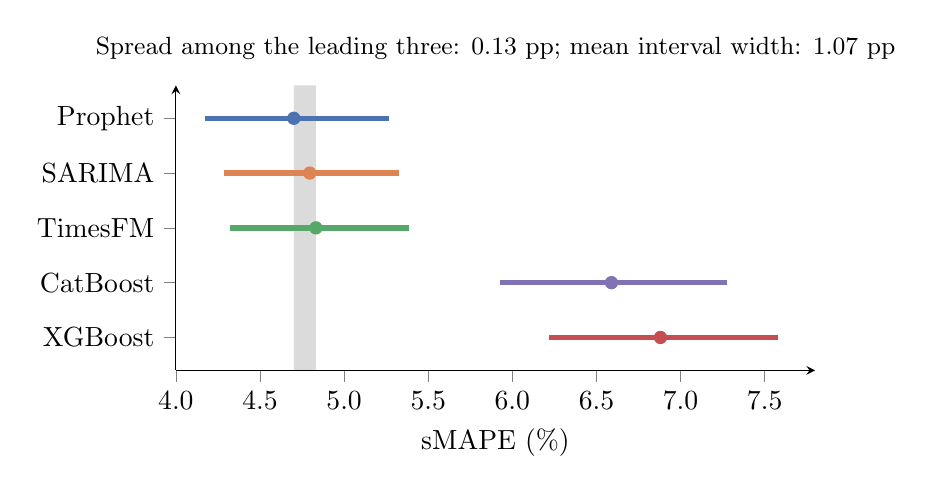
\begin{tikzpicture}
\begin{axis}[
  width=0.80\textwidth, height=5.2cm,
  xlabel={sMAPE (\%)}, xmin=4.0, xmax=7.8,
  xtick={4.0,4.5,5.0,5.5,6.0,6.5,7.0,7.5},
  xticklabel style={/pgf/number format/fixed, /pgf/number format/precision=1,
                     /pgf/number format/zerofill},
  ymin=0.4, ymax=5.6, ytick={5,4,3,2,1}, yticklabels={Prophet,SARIMA,TimesFM,CatBoost,XGBoost},
  axis lines=left, tick align=outside, tick pos=left,
  title style={align=left, font=\small},
  title={Spread among the leading three: 0.13 pp; mean interval width: 1.07 pp},
]
\addplot[draw=none, fill=black, fill opacity=0.14, forget plot]
  coordinates {(4.7010,0.4) (4.8325,0.4) (4.8325,5.6) (4.7010,5.6)}
  \closedcycle;
\addplot[draw=cprophet, line width=2.0pt, mark=none] coordinates {(4.1709,5) (5.2675,5)};
\addplot[only marks, mark=*, mark size=2.2pt, draw=cprophet, fill=cprophet] coordinates {(4.7010,5)};
\addplot[draw=csarima, line width=2.0pt, mark=none] coordinates {(4.2890,4) (5.3270,4)};
\addplot[only marks, mark=*, mark size=2.2pt, draw=csarima, fill=csarima] coordinates {(4.7957,4)};
\addplot[draw=ctimesfm, line width=2.0pt, mark=none] coordinates {(4.3245,3) (5.3851,3)};
\addplot[only marks, mark=*, mark size=2.2pt, draw=ctimesfm, fill=ctimesfm] coordinates {(4.8325,3)};
\addplot[draw=ccatboost, line width=2.0pt, mark=none] coordinates {(5.9248,2) (7.2734,2)};
\addplot[only marks, mark=*, mark size=2.2pt, draw=ccatboost, fill=ccatboost] coordinates {(6.5893,2)};
\addplot[draw=cxgboost, line width=2.0pt, mark=none] coordinates {(6.2170,1) (7.5794,1)};
\addplot[only marks, mark=*, mark size=2.2pt, draw=cxgboost, fill=cxgboost] coordinates {(6.8804,1)};
\end{axis}
\end{tikzpicture}
\caption{sMAPE by model with 95\% bootstrap intervals over rolling origin windows. Points
are the observed values, bars the intervals. The grey band spans the three leading models.
Its width is the quantity usually reported as a ranking; the bars are the uncertainty of
each estimate. Boosting models sit clearly apart, which is the one separation the data
support.}
\label{fig:smape}
\end{figure}

\subsection{Two models fail to beat a naive benchmark}\label{sec:naive}

A forecast is informative only relative to a rule that requires no model, and the scaled
error in Table~\ref{tab:desempenho} makes that comparison explicit. The seasonal naive
method, which simply repeats the same calendar month of the previous year, attains an sMAPE
of 6.27\% and a MASE of 1.148; adding a drift term brings it to 6.18\%. Prophet, SARIMA and
TimesFM sit far below that, at MASE 0.860, 0.880 and 0.887, reducing the error of the
seasonal benchmark by roughly a quarter. CatBoost and XGBoost sit above it, at 1.213 and
1.263, or 6.59\% and 6.88\% in sMAPE.

The unstructured naive method, which repeats the last observed month and ignores the annual
cycle, is far behind everything else at 10.74\%. The distance between it and the seasonal
naive method measures how much of this series is simply the annual cycle, and it is most of
what there is to forecast.

The claim these numbers support is that the two boosting models fail to improve on a rule
that requires no model, not that they are reliably worse than it. Applying the criterion
declared in Section~\ref{sec:metodos} to the comparison against the seasonal naive method,
neither difference qualifies: for CatBoost the paired interval is $[-0.056, +0.716]$ and no
Diebold-Mariano cell reaches significance, and for XGBoost the interval excludes zero but
again no cell does. The honest reading is that a decision maker offered these two models has
no evidence that either would beat repeating last year, which is a sufficient reason not to
pay for the complexity.

This does not follow from an unlucky hyperparameter choice. A separate tuning study using
Bayesian optimisation over 40 trials, with the search restricted to the first sixty months
so that no validation data enters any test window, moved CatBoost from 6.59\% to 6.42\%.
The same procedure applied to XGBoost moved it 0.13 pp in the wrong direction, from 6.88\%
to 7.02\%, leaving it worse than its own untuned configuration.
Table~\ref{tab:optuna} reports the search in full.
Repeating the CatBoost search over 60 trials with
the test windows deliberately exposed, an upper bound that no honest procedure can attain,
yields 6.35\%, and the same procedure applied to XGBoost yields 6.25\%. The CatBoost ceiling
remains behind the seasonal naive method; the XGBoost ceiling passes it, by 0.02 of a
percentage point. Neither observation changes the argument. A margin of two hundredths of a
point is an order of magnitude below the smallest difference this paper is willing to call
real, and both figures are the score of a configuration selected by reading the test set,
which bounds what tuning could buy rather than measuring what it does buy. Both ceilings
remain some 1.5 pp behind the three leading approaches.
The limitation is not the size of the search.

\subsection{The finding survives removing the pandemic}

\input{tables/tab8_covid}

The test period runs from January 2015 to December 2023 and therefore contains the pandemic,
whose level shocks could plausibly drive the comparison between models. Table~\ref{tab:covid}
removes it, in two ranges, because the choice of cut is arguable: an acute definition ending
with mass vaccination, and a wider one that also absorbs Omicron and the late excess
mortality. Whole windows are dropped rather than individual months, since the paired
bootstrap needs every model evaluated on the same rectangle of windows and horizons, and no
model is refitted, so the only thing that changes is which windows are scored.

Removing the pandemic makes every model better by about the same amount. Prophet improves
from 4.70\% to 3.60\% and 3.47\% under the two exclusions, and the other
two follow within a tenth of a point. This is the expected signature of a period that is
hard for everyone rather than of a period that favours one method.

The central finding does not move. In all three test periods, every pairwise difference among
Prophet, SARIMA and TimesFM contains zero and no Diebold-Mariano cell reaches significance,
0 of 6 in every comparison. Under the widest exclusion the ordering itself changes, with
SARIMA ahead of Prophet by 0.06 percentage points where it was behind by 0.10 in the full
period. A ranking that reverses when 41 of 103 windows are removed is not a ranking, which is
the same conclusion Table~\ref{tab:pares} reaches by a different route.

One number does move, and in the direction that matters for the boosting models. Their
disadvantage against the seasonal naive method widens once the pandemic is excluded, from
0.32 to 0.79 percentage points for CatBoost and from 0.61 to 1.12 for XGBoost, and
the paired intervals stop containing zero. The Diebold-Mariano requirement is still not met,
at 1 and 2 cells of six, so the conclusion of Section~\ref{sec:naive} stands unchanged rather
than strengthened: what the data support is the absence of evidence that boosting beats a
rule requiring no model, and the pandemic was not what was hiding it.

% gerado por scripts/revisao/build_revisao_tabs.py -- nao editar a mao
\begin{table}[htbp]
\centering
\small
\setlength{\tabcolsep}{4pt}
\caption{Hyperparameter search for the two gradient boosting models: the accuracy of the
untuned configuration reported in Table~\ref{tab:desempenho}, of an honest search, and of
a search allowed to see the test set. A positive gain means the search improved on the
untuned model.}
\label{tab:optuna}
\begin{tabular}{lrrrrrrr}
\toprule
& \multicolumn{3}{c}{sMAPE (\%)} & \multicolumn{2}{c}{Gain (pp)} & & \\
\cmidrule(lr){2-4} \cmidrule(lr){5-6}
Model & Untuned & Honest & Leaked & Honest & Leaked & Trials & Hours \\
\midrule
CatBoost & 6.59 & 6.42 & 6.35 & $+0.17$ & $+0.24$ & 40 + 60 & 2.1 \\
XGBoost & 6.88 & 7.02 & 6.25 & $-0.13$ & $+0.63$ & 40 + 60 & 1.1 \\
\midrule
Seasonal naive & \multicolumn{3}{c}{6.27} & --- & --- & --- & --- \\
\bottomrule
\end{tabular}

\vspace{0.5em}
\begin{minipage}{\textwidth}
\footnotesize
The honest column tunes on a development split carved out of the training data of each
origin, so no observation from the scored period is visible to the search; it is the column
that describes what tuning is worth. The leaked column selects the configuration by its
score on the test forecasts themselves. That is not a result, it is a bound: no search
without a time machine can do better. Both models were given the same budget, reported in
the last two columns as honest trials plus leaked trials and total wall clock. The honest
search buys CatBoost less than two tenths of a percentage point and costs XGBoost two
tenths, and neither honestly tuned model reaches the seasonal naive method of
6.27\%. The leaked column does reach it once, for XGBoost, by
0.019 of a percentage point. That margin is an
order of magnitude below anything this paper treats as a difference, and it is the
score of a configuration chosen by looking at the answer, so it bounds what tuning
could buy rather than showing what it does buy. All three columns are measured in
the environment pinned by the repository, so the gains compare like with like.
Even the leaked bound leaves both more than a percentage point behind the three leading
models of Table~\ref{tab:desempenho}. Under-tuning is therefore not the explanation for
the boosting results. The untuned column is the value the pinned environment produces, which for
XGBoost is 6.88\% rather than the
6.85\% of the environment where the search was first run: XGBoost does not
reproduce across library versions, a limitation already declared in the manuscript. The
CatBoost row reproduces its three original values exactly, which is what isolates that
limitation to one model.
\end{minipage}
\end{table}

\subsection{Feature engineering does not rescue the boosting models}

% gerado por scripts/build_paper_assets.py -- nao editar a mao
\begin{table}[htbp]
\centering
\small
\setlength{\tabcolsep}{4pt}
\caption{Feature engineering variants for the two gradient boosting models, evaluated under
the same protocol as Table~\ref{tab:desempenho}. The last two columns test the CatBoost
variant against the seasonal naive method.}
\label{tab:variantes}
\begin{tabular}{lrrrrcc}
\toprule
& \multicolumn{2}{c}{CatBoost} & \multicolumn{2}{c}{XGBoost}
& \multicolumn{2}{c}{CatBoost vs seasonal naive} \\
\cmidrule(lr){2-3} \cmidrule(lr){4-5} \cmidrule(lr){6-7}
Variant & sMAPE & MASE & sMAPE & MASE & 95\% CI of $\Delta$ & DM \\
\midrule
Lags only (as reported) & 6.59 & 1.213 & 6.88 & 1.263 & $[-0.06, +0.72]$ & 0/6 \\
+ rolling window statistics & 6.79 & 1.248 & 6.95 & 1.275 & $[+0.16, +0.90]$ & 0/6 \\
+ Fourier calendar terms & 6.27 & 1.150 & 6.61 & 1.214 & $[-0.37, +0.39]$ & 0/6 \\
Seasonal differencing & 6.20 & 1.142 & 6.35 & 1.166 & $[-0.37, +0.23]$ & 0/6 \\
Differencing + windows + calendar & 6.14 & 1.129 & 6.44 & 1.181 & $[-0.43, +0.14]$ & 0/6 \\
As above, direct multi-step & 6.09 & 1.126 & 6.39 & 1.183 & $[-0.45, +0.10]$ & 0/6 \\
\midrule
Seasonal naive (benchmark) & \multicolumn{4}{c}{6.27 \quad 1.148} & --- & --- \\
\bottomrule
\end{tabular}

\vspace{0.5em}
\begin{minipage}{\textwidth}
\footnotesize
The first row is the configuration reported in Table~\ref{tab:desempenho} and reproduces it.
Each subsequent row changes one thing. Adding rolling window statistics makes both models
worse. Replacing the raw level by the seasonal difference $y_t - y_{t-12}$ is the single
change that helps, and it helps because it hands the models the annual cycle instead of
requiring them to learn it. The best variant, CatBoost with differencing, calendar terms and
one model per horizon, reaches 6.09\% against
6.27\% for the seasonal naive method. That difference does not meet the
criterion declared in Section~\ref{sec:metodos}: the paired bootstrap interval is
$[-0.45,
+0.10]$ and contains zero, and no
Diebold-Mariano cell of six reaches significance. $\Delta$ is the difference in sMAPE
against the seasonal naive method, so negative favours the variant. Every variant remains
more than one percentage point behind the three leading models of
Table~\ref{tab:desempenho}.
\end{minipage}
\end{table}

The configuration in Table~\ref{tab:desempenho} gives the boosting models twelve lags of the
target and nothing else, which is a thin representation for a series whose dominant structure
is an annual cycle. Table~\ref{tab:variantes} asks whether a richer one changes the verdict,
changing one thing at a time under the same protocol.

It does not, and the pattern of what helps is more informative than the totals. Adding
rolling window statistics, the most common reflex when a tree model underperforms on a time
series, makes both models worse. Adding Fourier calendar terms helps. The largest single
gain comes from forecasting the seasonal difference $y_t - y_{t-12}$ and reconstructing the
level afterwards, which improves CatBoost from 6.59\% to 6.20\%. The interpretation is
direct: what the boosting models were failing at was representing the annual cycle, and the
transformations that help are the ones that supply it rather than the ones that add capacity.

The best variant combines all of it with one model per horizon and reaches 6.09\%,
against 6.27\% for the seasonal naive method. Taken as a point estimate that reverses the
comparison, and it is the number a reader would quote. It does not survive the criterion
this paper applies everywhere else: the paired bootstrap interval on the difference is
$[-0.45, +0.10]$, which contains zero, and none of the six Diebold-Mariano
cells reaches significance. After six variants and two model families, there is still no
configuration of gradient boosting here that can be shown to beat repeating the previous
year, and every one of them remains more than a percentage point behind Prophet, SARIMA and
TimesFM.

\subsection{A tabular foundation model narrows the gap without closing it}

The two boosting models are not the strongest tabular learners available, and a comparison
that concludes against tabular methods while omitting the current state of the art would be
incomplete. TabPFN, a transformer pre-trained on synthetic tabular tasks, was therefore run
under the identical protocol: the same 103 windows, the same six-month horizon, the same
twelve lags of the target as the only inputs.

It reaches an sMAPE of 5.85\%, ahead of CatBoost by 0.74 percentage points and of XGBoost by
1.03, making it the strongest tabular model tested here. It sits ahead of both naive
references on the point estimate, at 6.18\% and 6.27\%, and behind the three leading models
by more than 1.0 percentage point.

It is the comparison against the naive references that decides what this row means, and
here the paired test was run rather than deferred. Against the seasonal naive method the
advantage is 0.42 percentage points with a
paired interval of $[-0.698, -0.128]$ that excludes zero, and against the seasonal naive
with annual drift it is 0.33 points with $[-0.622, -0.031]$, also excluding zero. This is a
stronger result than any boosting variant obtained: the best of them, at a margin of 0.18
points over the same benchmark, produced an interval of $[-0.45, +0.10]$ that contains zero.
The criterion declared in Section~\ref{sec:metodos} nonetheless is not met, because it
requires agreement between the interval and the horizon-level tests, and the
Diebold-Mariano test reaches significance in only one of six cells against each seasonal
benchmark.

The distribution of that single cell is more informative than the aggregate. Significance
is confined to the one-month horizon ($p=0.0012$ against the seasonal naive method and
$p=0.0044$ against the drift variant) and the differential decays thereafter, with $p$
above 0.35 from the third horizon onward in both comparisons. The advantage of the tabular
foundation model over seasonal persistence is therefore a one-month-ahead advantage, and it
does not survive the six-month horizon this paper is about. Reported as such, the finding is
neither a defeat of the naive benchmark nor a null: it is a horizon-dependent gain that the
pre-declared criterion, by design, declines to call established.

One caveat applies to this row and to no other in the paper. TabPFN was evaluated through a
hosted inference API, so the model version is not captured by the pinned environment that
fixes every other result here. The same protocol returned 6.04\% under an earlier client
release and 5.85\% under the current one, a shift of 0.19 percentage points, larger than the
version sensitivity that motivated pinning the environment in the first place. This number
is a dated measurement rather than a quantity a reader can reproduce from the repository,
and it should be read accordingly.

The reviewer's request is nonetheless answered, and answered against the reviewer's
expectation: including the strongest tabular learner does not change the conclusion. The
distance from TabPFN to Prophet is 1.14 percentage points, wider than the entire spread
among the three leading models, and the Diebold-Mariano test places SARIMA ahead of it in
four of six horizons. What the boosting results were showing was not the absence
of a good tabular model but the nature of the task: 168 monthly observations dominated by a
clean annual cycle do not reward this class of method.

\subsection{The prediction intervals are not calibrated}

\input{tables/tab6_calibracao}

Two of the five models produce prediction intervals natively, and Table~\ref{tab:calibracao}
reports what those intervals are worth. At a nominal 95\%, SARIMA covers 84.5\% of
observations and Prophet 77.2\%. Both undercover, by 10.5 and 17.8 percentage points
respectively, so an interval presented to a manager as containing the outcome nineteen times
in twenty would in fact contain it roughly seventeen times in twenty for SARIMA and fifteen
for Prophet.

The two failures are not the same failure. Prophet's intervals are the narrower of the two,
1045 against 1288 deaths per month, and they are not better placed, so it pays for the width
with misses: its interval score is 4468 against SARIMA's 3500. Its coverage also decays with
the forecast horizon, from 0.796 at one month to 0.748 at six, while SARIMA stays close to
flat between 0.854 and 0.835. Prophet has the lowest sMAPE of all five models and the worse
of the two intervals; ranking by point accuracy and ranking by interval quality disagree,
which is a reason not to select a model for operational use on point accuracy alone.

These intervals come from the same fitted models reported in
Table~\ref{tab:desempenho}: the point forecasts produced alongside the intervals were checked
against the stored benchmark forecasts before the coverage was computed. What is measured
here is therefore the calibration of the models this paper reports, not of models sharing
their names.

\subsection{The leading three models are indistinguishable}

The spread in sMAPE among Prophet, SARIMA and TimesFM is 0.13 pp, against a mean interval
width of 1.07 pp, a ratio of 0.12. Table~\ref{tab:pares} shows that all three paired
differences contain zero and that no Diebold-Mariano cell reaches significance, 0 of 18.

\input{tables/tab2_pares}

In our earlier round on 60 months, the point ranking placed TimesFM first (7.30\%) and
Prophet last (7.68\%), a spread of 0.38 pp against a mean interval width of 2.45 pp.
Extending the series inverted that ordering while narrowing the intervals by a factor of
2.3. An ordering that reverses when more data arrive, and whose intervals overlap in both
rounds, is not a finding about the models.

\subsection{Boosting is detectably worse}

XGBoost and CatBoost sit 1.76 pp or more above the leading group. All 36 comparisons of a
boosting model against one of the leading three reach $p<0.05$ on the Diebold-Mariano test,
and the bootstrap $p$ for each pooled difference is below 0.001. Unlike the ordering within
the leading group, this separation is established under the pre-declared criterion.
Recursive boosting over lags, without exogenous information, is not competitive on this
series.

\subsection{Training history dominates model choice}

\input{tables/tab3_serie}

Table~\ref{tab:serie} restricts attention to the test dates shared with the earlier round.
Nine additional years of training reduce error by 1.23 to 1.71 pp on identical targets,
roughly ten times the 0.13 pp separating the models here and four times the 0.38 pp that
separated them before. Within the options available to a practitioner, extending the series
was worth far more than exchanging the model.

\subsection{The foundation model's advantage is robustness to short history}

% gerado por scripts/build_paper_assets.py -- nao editar a mao
\begin{table}[htbp]
\centering
\small
\setlength{\tabcolsep}{4pt}
\caption{Expanding versus sliding 60-month training window, evaluated on identical
test origins. A negative difference means the expanding window is more accurate.}
\label{tab:janela}
\begin{tabular}{lrrrcrc}
\toprule
Model & Expanding & Sliding 60 & Diff. (pp) & 95\% CI & $p$ & DM cells $p<0.05$ \\
\midrule
Prophet & 4.70 & 5.39 & $-0.69$ & $[-1.159, -0.219]$ & 0.005 & 0 of 6 \\
SARIMA & 4.80 & 5.46 & $-0.66$ & $[-1.008, -0.346]$ & 0.000 & 3 of 6 \\
TimesFM & 4.83 & 4.74 & $+0.09$ & $[-0.125, +0.307]$ & 0.424 & 0 of 6 \\
CatBoost & 6.59 & 6.64 & $-0.05$ & $[-0.288, +0.176]$ & 0.661 & 0 of 6 \\
XGBoost & 6.88 & 6.86 & $+0.02$ & $[-0.258, +0.303]$ & 0.879 & 0 of 6 \\
\midrule
CatBoost, enriched & 6.09 & 6.59 & $-0.50$ & --- & --- & --- \\
XGBoost, enriched & 6.39 & 6.79 & $-0.41$ & --- & --- & --- \\
\bottomrule
\end{tabular}

\vspace{0.5em}
\begin{minipage}{\textwidth}
\footnotesize
The only difference between the two runs is how much past each model may use: the
expanding window trains from the start of the series to the origin (60 to 162 months),
the sliding window on the most recent 60 months only. Test origins, horizons and
evaluation are identical, so the bootstrap is paired by window. Under the pre-declared
criterion, only SARIMA meets both conditions. The two rows below the second rule are the best feature engineering variant of each boosting model (seasonal differencing, calendar terms, one model per horizon; Table~\ref{tab:variantes}), run under both window policies. They lose 0.41 to 0.50 percentage points under the short window, so the advantage of feature engineering does not survive a short history either. Their interval, $p$ and DM cells are left blank because only the aggregate metrics of the sliding run were retained, not its individual forecasts, and the paired bootstrap needs the forecasts.
\end{minipage}
\end{table}


Table~\ref{tab:janela} and Figure~\ref{fig:janela} isolate the value of long history for
each model. Discarding history beyond five years costs SARIMA 0.66 pp, the only comparison
in this study that meets the pre-declared criterion in full, and costs Prophet 0.69 pp with
an interval excluding zero but no horizon-level significance. TimesFM is unaffected
($+0.09$ pp, $p=0.42$), consistent with a bounded context window, internal normalisation
and knowledge acquired in pre-training rather than from the target series. In the truncated
regime TimesFM leads at 4.74\% against 5.46\% for SARIMA.

\begin{figure}[htbp]
\centering
% gerado por scripts/build_paper_assets.py -- nao editar a mao
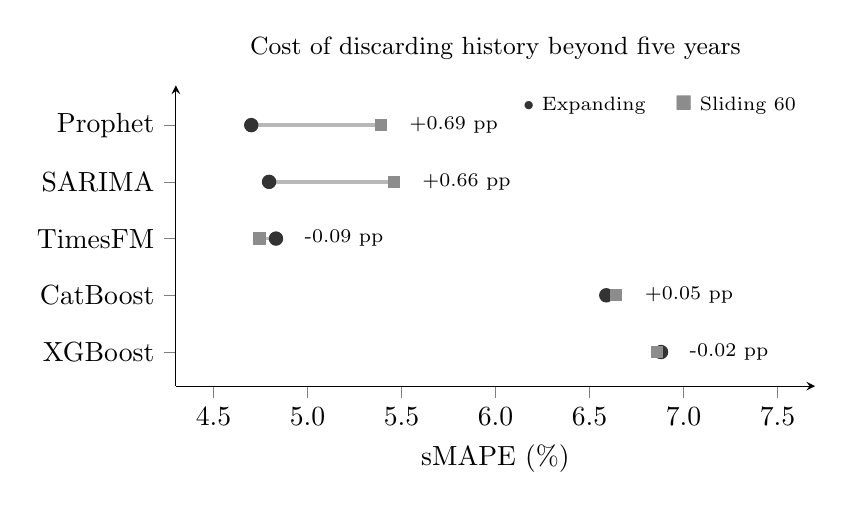
\begin{tikzpicture}
\begin{axis}[
  width=0.80\textwidth, height=5.4cm,
  xlabel={sMAPE (\%)}, xmin=4.3, xmax=7.7,
  xtick={4.5,5.0,5.5,6.0,6.5,7.0,7.5},
  xticklabel style={/pgf/number format/fixed, /pgf/number format/precision=1,
                     /pgf/number format/zerofill},
  ymin=0.4, ymax=5.7, ytick={5,4,3,2,1}, yticklabels={Prophet,SARIMA,TimesFM,CatBoost,XGBoost},
  axis lines=left, tick align=outside, tick pos=left,
  title style={align=left, font=\small},
  title={Cost of discarding history beyond five years},
]
\addplot[draw=black!28, line width=1.2pt, mark=none] coordinates {(4.7010,5) (5.3909,5)};
\addplot[only marks, mark=*, mark size=2.4pt, draw=black!80, fill=black!80] coordinates {(4.7010,5)};
\addplot[only marks, mark=square*, mark size=2.0pt, draw=black!45, fill=black!45] coordinates {(5.3909,5)};
\node[anchor=west, font=\scriptsize, text=black] at (axis cs:5.4909,5) {+0.69 pp};
\addplot[draw=black!28, line width=1.2pt, mark=none] coordinates {(4.7957,4) (5.4588,4)};
\addplot[only marks, mark=*, mark size=2.4pt, draw=black!80, fill=black!80] coordinates {(4.7957,4)};
\addplot[only marks, mark=square*, mark size=2.0pt, draw=black!45, fill=black!45] coordinates {(5.4588,4)};
\node[anchor=west, font=\scriptsize, text=black] at (axis cs:5.5588,4) {+0.66 pp};
\addplot[draw=black!28, line width=1.2pt, mark=none] coordinates {(4.8325,3) (4.7447,3)};
\addplot[only marks, mark=*, mark size=2.4pt, draw=black!80, fill=black!80] coordinates {(4.8325,3)};
\addplot[only marks, mark=square*, mark size=2.0pt, draw=black!45, fill=black!45] coordinates {(4.7447,3)};
\node[anchor=west, font=\scriptsize, text=black] at (axis cs:4.9325,3) {-0.09 pp};
\addplot[draw=black!28, line width=1.2pt, mark=none] coordinates {(6.5893,2) (6.6424,2)};
\addplot[only marks, mark=*, mark size=2.4pt, draw=black!80, fill=black!80] coordinates {(6.5893,2)};
\addplot[only marks, mark=square*, mark size=2.0pt, draw=black!45, fill=black!45] coordinates {(6.6424,2)};
\node[anchor=west, font=\scriptsize, text=black] at (axis cs:6.7424,2) {+0.05 pp};
\addplot[draw=black!28, line width=1.2pt, mark=none] coordinates {(6.8804,1) (6.8569,1)};
\addplot[only marks, mark=*, mark size=2.4pt, draw=black!80, fill=black!80] coordinates {(6.8804,1)};
\addplot[only marks, mark=square*, mark size=2.0pt, draw=black!45, fill=black!45] coordinates {(6.8569,1)};
\node[anchor=west, font=\scriptsize, text=black] at (axis cs:6.9804,1) {-0.02 pp};
\node[anchor=east, font=\scriptsize, text=black] at (axis cs:7.65,5.35)
  {\textcolor{black!80}{$\bullet$} Expanding \quad
    \textcolor{black!45}{$\blacksquare$} Sliding 60};
\end{axis}
\end{tikzpicture}
\caption{Accuracy under an expanding training window and under a sliding 60-month window,
on identical test origins. The classical models degrade when history is truncated; the
foundation model does not, and overtakes them in that regime. The annotation on each row
is the cost of truncating, sliding minus expanding, so a positive value means the model
loses accuracy when older history is discarded; Table~\ref{tab:janela} reports the same
pairs with the opposite subtraction.}
\label{fig:janela}
\end{figure}

Error decomposed by forecast horizon (Figure~\ref{fig:horizonte}) shows the leading three
models interleaving at every horizon, with the boosting models separated throughout.

\begin{figure}[htbp]
\centering
% gerado por scripts/build_paper_assets.py -- nao editar a mao
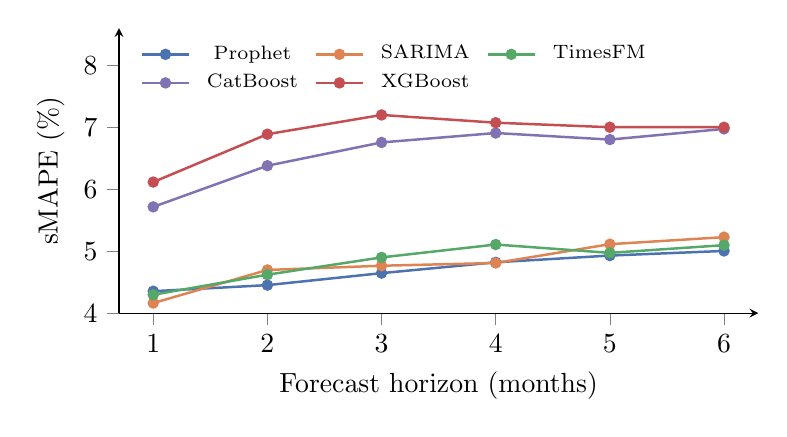
\begin{tikzpicture}
\begin{axis}[
  width=0.80\textwidth, height=5.2cm,
  xlabel={Forecast horizon (months)}, ylabel={sMAPE (\%)},
  xmin=0.7, xmax=6.3, xtick={1,2,3,4,5,6},
  axis lines=left, tick align=outside, tick pos=left,
  legend style={at={(0.02,0.98)}, anchor=north west, draw=none, fill=none,
                 font=\scriptsize, legend columns=3, column sep=4pt},
  ymin=4, ymax=8.6, ytick={4,5,6,7,8},
  % Sem o ymin e o ytick explicitos, a escolha automatica punha a marca mais baixa em
  % 5 e os tres modelos lideres ficavam abaixo dela, sem nenhuma referencia de leitura,
  % com o ponto do SARIMA em h=1 encostado no eixo.
]
\addplot[draw=cprophet, mark=*, mark size=1.6pt, line width=0.9pt, mark options={draw=cprophet, fill=cprophet}] coordinates {(1,4.3538) (2,4.4520) (3,4.6456) (4,4.8209) (5,4.9294) (6,5.0041)};
\addplot[draw=csarima, mark=*, mark size=1.6pt, line width=0.9pt, mark options={draw=csarima, fill=csarima}] coordinates {(1,4.1625) (2,4.6971) (3,4.7652) (4,4.8096) (5,5.1129) (6,5.2266)};
\addplot[draw=ctimesfm, mark=*, mark size=1.6pt, line width=0.9pt, mark options={draw=ctimesfm, fill=ctimesfm}] coordinates {(1,4.2967) (2,4.6208) (3,4.8998) (4,5.1074) (5,4.9729) (6,5.0975)};
\addplot[draw=ccatboost, mark=*, mark size=1.6pt, line width=0.9pt, mark options={draw=ccatboost, fill=ccatboost}] coordinates {(1,5.7154) (2,6.3801) (3,6.7560) (4,6.9079) (5,6.8022) (6,6.9744)};
\addplot[draw=cxgboost, mark=*, mark size=1.6pt, line width=0.9pt, mark options={draw=cxgboost, fill=cxgboost}] coordinates {(1,6.1161) (2,6.8891) (3,7.1997) (4,7.0746) (5,7.0017) (6,7.0013)};
\legend{Prophet,SARIMA,TimesFM,CatBoost,XGBoost}
\end{axis}
\end{tikzpicture}
\caption{sMAPE by forecast horizon, $n=103$ windows per cell. The leading three models
cross repeatedly, which is the horizon-level counterpart of the pooled result in
Table~\ref{tab:pares}.}
\label{fig:horizonte}
\end{figure}

\subsection{Temperature supplies the calendar, and clears the threshold once}

% gerado por scripts/build_paper_assets.py -- nao editar a mao
\begin{table}[htbp]
\centering
\small
\setlength{\tabcolsep}{4pt}
\caption{Effect of monthly minimum temperature as an exogenous covariate, under the
leakage-free climatology policy, and the labelled ceiling scenario. Prophet is
included through its native \texttt{add\_regressor} interface; TimesFM, which has
no such interface in this implementation, is not.}
\label{tab:temperatura}
\begin{tabular}{lrrrcrr}
\toprule
Model & Without & With temp. & Gain (pp) & 95\% CI & DM cells $p<0.05$ & Ceiling \\
\midrule
Prophet & 4.70 & 4.74 & $-0.035$ & $[-0.081, +0.013]$ & 0 of 6 & 4.63 \\
SARIMA & 4.80 & 4.66 & $+0.136$ & $[+0.034, +0.257]$ & 1 of 6 & 4.63 \\
CatBoost & 6.59 & 6.33 & $+0.258$ & $[+0.073, +0.452]$ & 1 of 6 & 6.30 \\
XGBoost & 6.88 & 6.51 & $+0.368$ & $[+0.190, +0.548]$ & 3 of 6 & 6.53 \\
\bottomrule
\end{tabular}

\vspace{0.5em}
\begin{minipage}{\textwidth}
\footnotesize
Under the climatology policy the future covariate is the month-of-year mean recomputed
for each window from the exogenous series truncated at that window's training end, so no
value from after the training end is visible. The ceiling column replaces it with the
true observed future temperature, which leaks by construction and is reported only to
bound what a perfect weather forecast could add. Gain is positive when temperature helps.
The three gains that exclude zero are SARIMA, CatBoost and XGBoost, but none reaches the
pre-declared threshold of DM significance in at least three horizons, so the effect is
reported as suggestive and not established. Prophet is included through add\_regressor(); its baseline run reproduces the forecasts of Table~\ref{tab:desempenho} exactly, so the two rows describe the same model with and without the covariate. It is the one model the covariate does not help: the gain is negative and its interval spans zero.
TimesFM does not accept exogenous regressors in this implementation and was excluded from
this comparison rather than being given an input it would ignore.
\end{minipage}
\end{table}


Prophet is the one model for which the covariate makes the forecast worse, by 0.035
percentage points, and that difference is not significant either: the paired interval is
$[-0.081, +0.013]$ and no Diebold-Mariano cell reaches significance. Since Prophet already
fits an explicit annual seasonality, minimum temperature supplies it with a noisier version
of a signal it has already extracted from the target. The same reading applies in the other
direction to the boosting models, whose gain from the covariate is the largest of the four:
what temperature adds for them is the seasonality their twelve lags were failing to
represent, which is the same conclusion reached in Table~\ref{tab:variantes} by a different
route.

XGBoost is the only row of the four that meets the criterion of Section~\ref{sec:metodos}: its
gain of 0.368 percentage points has a paired interval of $[+0.190, +0.548]$ that excludes
zero, and 3 of the six Diebold-Mariano cells reach significance. This is the one place in
this paper where the covariate can be said to help rather than to appear to help, and it helps
the model that needed it most while leaving it still the weakest of the five.

\input{tables/revisao_tab_temp_diffcal}

That reading is a claim about mechanism, and it is falsifiable, so it was tested. If the
covariate helps the boosting models because it supplies a seasonality their features lack,
then giving them an explicit calendar term should absorb most of the gain; if the gain
survives, the covariate is carrying weather information beyond climatology and the
explanation is wrong. Table~\ref{tab:tempdiffcal} repeats the comparison with Fourier calendar terms
added to the feature set. It shrinks the CatBoost gain from 0.258 to 0.076 percentage points,
and turns the XGBoost gain from +0.327 to -0.036, a change of sign. The latter figure is
within a thousandth of a point of what Prophet, which fits an explicit annual seasonality of
its own, records in Table~\ref{tab:temperatura}. Two models that arrive at explicit
seasonality by different routes are hurt by the covariate by the same amount, which is the
prediction the explanation makes and not one it could have made if it were wrong. Minimum
temperature in this series is close to a deterministic function of the calendar month, and
what it was adding to the boosting models was the calendar.

\begin{figure}[htbp]
\centering
% gerado por scripts/build_paper_assets.py -- nao editar a mao
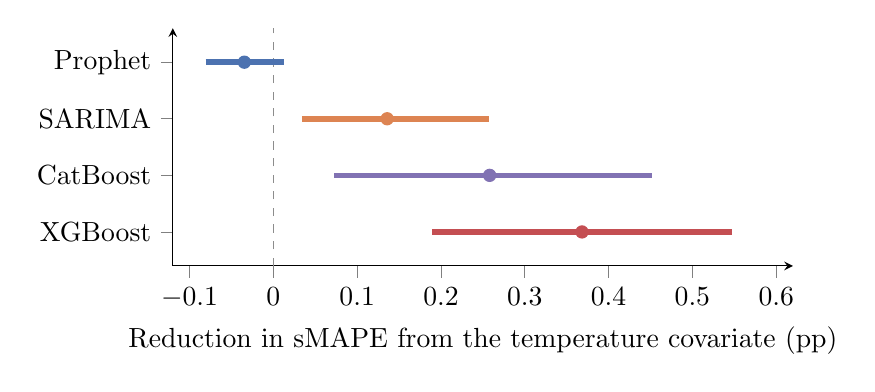
\begin{tikzpicture}
\begin{axis}[
  width=0.78\textwidth, height=4.6cm,
  xlabel={Reduction in sMAPE from the temperature covariate (pp)},
  xmin=-0.12, xmax=0.62,
  % com valores pequenos o pgfplots gera tick automatico em notacao cientifica
  % (-5 \cdot 10^-2) e os rotulos colidem. Tick e formato explicitos.
  xtick={-0.1,0,0.1,0.2,0.3,0.4,0.5,0.6},
  scaled x ticks=false,
  xticklabel style={/pgf/number format/fixed, /pgf/number format/precision=1},
  ymin=0.4, ymax=4.6, ytick={4,3,2,1}, yticklabels={Prophet,SARIMA,CatBoost,XGBoost},
  axis lines=left, tick align=outside, tick pos=left,
]
\draw[black!45, dashed, line width=0.6pt]
  (axis cs:0,0.4) -- (axis cs:0,4.6);
\addplot[draw=cprophet, line width=2.0pt, mark=none] coordinates {(-0.0808,4) (0.0129,4)};
\addplot[only marks, mark=*, mark size=2.2pt, draw=cprophet, fill=cprophet] coordinates {(-0.0346,4)};
\addplot[draw=csarima, line width=2.0pt, mark=none] coordinates {(0.0340,3) (0.2573,3)};
\addplot[only marks, mark=*, mark size=2.2pt, draw=csarima, fill=csarima] coordinates {(0.1358,3)};
\addplot[draw=ccatboost, line width=2.0pt, mark=none] coordinates {(0.0728,2) (0.4519,2)};
\addplot[only marks, mark=*, mark size=2.2pt, draw=ccatboost, fill=ccatboost] coordinates {(0.2581,2)};
\addplot[draw=cxgboost, line width=2.0pt, mark=none] coordinates {(0.1898,1) (0.5476,1)};
\addplot[only marks, mark=*, mark size=2.2pt, draw=cxgboost, fill=cxgboost] coordinates {(0.3683,1)};
\end{axis}
\end{tikzpicture}
\caption{Reduction in sMAPE from adding monthly minimum temperature as an exogenous
covariate under the leakage-free climatology policy, with 95\% paired bootstrap intervals.
Positive values favour the model with temperature. The four models are ordered by how much
seasonal structure their specification already carries, and the gain grows as that
structure falls away: it is negative for Prophet, which fits an explicit annual
seasonality, and largest for the two boosting models, whose only inputs are twelve lags.
Three intervals exclude zero, but only XGBoost also reaches the pre-declared horizon-level
threshold, so it is the one row reported as established rather than suggestive.}
\label{fig:temp}
\end{figure}

Across Table~\ref{tab:temperatura} and Figure~\ref{fig:temp}, then, the covariate divides
the models rather than lifting them together. All three positive gains have intervals
excluding zero, but only XGBoost also clears the horizon-level requirement; for SARIMA and
CatBoost, at 1 of six cells each, the effect remains suggestive and not established.

What the ceiling scenario adds is a limit on how much better any of this could get.
Replacing the climatological future covariate with the true observed future temperature,
which no operational forecast could access, improves SARIMA by a further 0.03 pp only. The
predictive content of monthly temperature in this series is therefore almost entirely its
climatology, information a seasonal model already carries, which is why the one model the
covariate demonstrably helps is the one whose features carried no calendar at all.

\subsection{Seasonality}

\begin{figure}[htbp]
\centering
% gerado por scripts/build_paper_assets.py -- nao editar a mao
\begin{tikzpicture}
\begin{axis}[
  width=0.80\textwidth, height=4.8cm,
  axis y line*=left, axis x line*=bottom,
  xmin=0.5, xmax=12.5, xtick={1,...,12}, xticklabels={J,F,M,A,M,J,J,A,S,O,N,D},
  ylabel={Mean deaths per month}, ylabel style={text=black},
  scaled y ticks=false, ytick={6500,7000,7500,8000},
  yticklabel style={text=black, /pgf/number format/fixed,
                     /pgf/number format/1000 sep={,}},
  tick align=outside,
  legend style={at={(0,1.03)}, anchor=south west, draw=none, fill=none,
                 font=\scriptsize, text=black},
]
\addplot[draw=black!80, mark=*, mark size=2.0pt, line width=1.1pt]
  coordinates {(1,6969.9) (2,6272.8) (3,6856.3) (4,6764.0) (5,7678.1) (6,7971.6) (7,8247.2) (8,7893.4) (9,7268.9) (10,7201.0) (11,6817.7) (12,7018.1)};
\addlegendentry{Deaths per month}
\end{axis}
\begin{axis}[
  width=0.80\textwidth, height=4.8cm,
  axis y line*=right, axis x line=none,
  xmin=0.5, xmax=12.5,
  ylabel={Mean minimum temperature ($^\circ$C)}, ylabel style={text=black},
  yticklabel style={text=black},
  tick align=outside,
  legend style={at={(1,1.03)}, anchor=south east, draw=none, fill=none,
                 font=\scriptsize, text=black},
]
\addplot[draw=ctemp, mark=square*, mark size=1.7pt, line width=0.9pt, dashed,
         mark options={draw=ctemp, fill=ctemp, solid}]
  coordinates {(1,19.72) (2,19.79) (3,19.16) (4,17.54) (5,15.07) (6,14.06) (7,13.44) (8,13.83) (9,15.76) (10,16.93) (11,17.33) (12,19.14)};
\addlegendentry{Minimum temperature}
\end{axis}
\end{tikzpicture}
\caption{Mean cardiovascular deaths by month of year (left axis) against mean monthly
minimum temperature (right axis), 2010--2023. The mortality peak coincides with the
temperature trough.}
\label{fig:sazonal}
\end{figure}

The series shows a stable seasonal pattern across all fourteen years, peaking in July
(mean 8{,}247 deaths) and reaching its trough in February (mean 6{,}273), an amplitude of
27.2\% around the mean (Figure~\ref{fig:sazonal}). The COVID-19 period introduced level
anomalies without disrupting the seasonal shape (Figure~\ref{fig:serie}).

\begin{figure}[htbp]
\centering
% gerado por scripts/build_paper_assets.py -- nao editar a mao
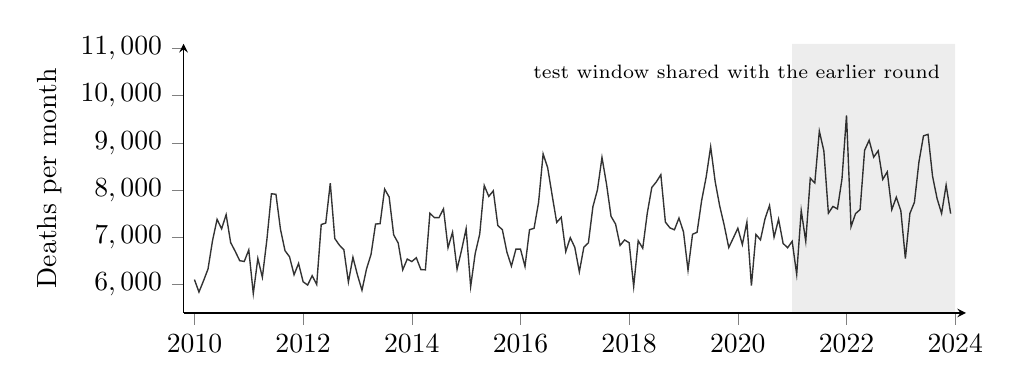
\begin{tikzpicture}
\begin{axis}[
  width=0.95\textwidth, height=5.0cm,
  xlabel={}, ylabel={Deaths per month},
  xmin=2009.8, xmax=2024.2, ymin=5400, ymax=11100,
  xtick={2010,2012,2014,2016,2018,2020,2022,2024},
  xticklabel style={/pgf/number format/1000 sep=},
  % sem isto o pgfplots troca o eixo por \cdot 10^4, que e ilegivel aqui
  scaled y ticks=false,
  ytick={6000,7000,8000,9000,10000,11000},
  yticklabel style={/pgf/number format/fixed, /pgf/number format/1000 sep={,}},
  axis lines=left, tick align=outside, tick pos=left,
  every axis plot/.append style={line width=0.5pt},
]
\addplot[draw=black!80, mark=none] coordinates {(2010.0000,6107) (2010.0833,5843) (2010.1667,6079) (2010.2500,6332) (2010.3333,6934) (2010.4167,7382) (2010.5000,7182) (2010.5833,7481) (2010.6667,6890) (2010.7500,6706) (2010.8333,6507) (2010.9167,6490) (2011.0000,6735) (2011.0833,5811) (2011.1667,6554) (2011.2500,6156) (2011.3333,6952) (2011.4167,7924) (2011.5000,7913) (2011.5833,7172) (2011.6667,6719) (2011.7500,6590) (2011.8333,6208) (2011.9167,6448) (2012.0000,6060) (2012.0833,5991) (2012.1667,6189) (2012.2500,6004) (2012.3333,7272) (2012.4167,7304) (2012.5000,8148) (2012.5833,6976) (2012.6667,6837) (2012.7500,6738) (2012.8333,6054) (2012.9167,6579) (2013.0000,6205) (2013.0833,5881) (2013.1667,6331) (2013.2500,6640) (2013.3333,7283) (2013.4167,7291) (2013.5000,8023) (2013.5833,7855) (2013.6667,7054) (2013.7500,6880) (2013.8333,6314) (2013.9167,6542) (2014.0000,6488) (2014.0833,6569) (2014.1667,6318) (2014.2500,6313) (2014.3333,7512) (2014.4167,7418) (2014.5000,7417) (2014.5833,7605) (2014.6667,6781) (2014.7500,7110) (2014.8333,6327) (2014.9167,6734) (2015.0000,7184) (2015.0833,5958) (2015.1667,6658) (2015.2500,7069) (2015.3333,8099) (2015.4167,7868) (2015.5000,7986) (2015.5833,7251) (2015.6667,7163) (2015.7500,6690) (2015.8333,6392) (2015.9167,6753) (2016.0000,6753) (2016.0833,6385) (2016.1667,7164) (2016.2500,7192) (2016.3333,7743) (2016.4167,8767) (2016.5000,8479) (2016.5833,7890) (2016.6667,7317) (2016.7500,7426) (2016.8333,6700) (2016.9167,6994) (2017.0000,6788) (2017.0833,6271) (2017.1667,6794) (2017.2500,6884) (2017.3333,7651) (2017.4167,8009) (2017.5000,8694) (2017.5833,8130) (2017.6667,7446) (2017.7500,7282) (2017.8333,6830) (2017.9167,6946) (2018.0000,6886) (2018.0833,5960) (2018.1667,6930) (2018.2500,6769) (2018.3333,7511) (2018.4167,8057) (2018.5000,8175) (2018.5833,8328) (2018.6667,7325) (2018.7500,7202) (2018.8333,7161) (2018.9167,7409) (2019.0000,7117) (2019.0833,6307) (2019.1667,7067) (2019.2500,7108) (2019.3333,7776) (2019.4167,8274) (2019.5000,8919) (2019.5833,8180) (2019.6667,7664) (2019.7500,7254) (2019.8333,6785) (2019.9167,6987) (2020.0000,7194) (2020.0833,6848) (2020.1667,7324) (2020.2500,5978) (2020.3333,7062) (2020.4167,6948) (2020.5000,7392) (2020.5833,7678) (2020.6667,7005) (2020.7500,7385) (2020.8333,6872) (2020.9167,6781) (2021.0000,6917) (2021.0833,6217) (2021.1667,7569) (2021.2500,6917) (2021.3333,8253) (2021.4167,8153) (2021.5000,9251) (2021.5833,8830) (2021.6667,7512) (2021.7500,7656) (2021.8333,7603) (2021.9167,8237) (2022.0000,9582) (2022.0833,7227) (2022.1667,7504) (2022.2500,7589) (2022.3333,8846) (2022.4167,9057) (2022.5000,8699) (2022.5833,8834) (2022.6667,8228) (2022.7500,8388) (2022.8333,7588) (2022.9167,7850) (2023.0000,7563) (2023.0833,6551) (2023.1667,7507) (2023.2500,7745) (2023.3333,8600) (2023.4167,9151) (2023.5000,9183) (2023.5833,8297) (2023.6667,7823) (2023.7500,7507) (2023.8333,8107) (2023.9167,7504)};
\addplot[draw=none, fill=black, fill opacity=0.07, forget plot]
  coordinates {(2021.0,5400) (2024.0,5400) (2024.0,11100) (2021.0,11100)} \closedcycle;
% ancorado a direita e dentro do limite do eixo: centralizado em 2022.5 o rotulo
% estourava a borda e saia cortado
\node[anchor=east, font=\scriptsize, text=black]
  at (axis cs:2023.9,10500) {test window shared with the earlier round};
\end{axis}
\end{tikzpicture}
\caption{Monthly cardiovascular deaths in the state of S\~ao Paulo, January 2010 to
December 2023 (168 months). The shaded region marks the test window shared with our
earlier 60-month round, used for the paired comparison in Table~\ref{tab:serie}.}
\label{fig:serie}
\end{figure}

\section{Discussion}

Among Prophet, SARIMA and TimesFM there is no detectable difference in forecasting monthly
cardiovascular mortality, and the ordering we ourselves reported on a shorter series
survived neither more data nor the addition of intervals. What did move accuracy was the
length of the training series, by roughly an order of magnitude more than the choice of
model.

\subsection{Rankings without intervals are not findings}

Our earlier round reported TimesFM first by 0.38 pp of sMAPE. That gap was smaller than the
interval of any single model by a factor of six, and the ordering reversed when the series
was extended. Had it been published as a ranking, it would have made a claim that the same
pipeline contradicted weeks later using more data.

This is not specific to our series. Backtesting forecasts from overlapping windows are
strongly dependent, and aggregate error over a few hundred such forecasts carries an
interval on the order of a percentage point, while published gaps between modern
forecasting methods are frequently a few tenths. Comparisons in this regime that report
only point estimates are underpowered by construction. Reporting the width of the interval
alongside the gap, and treating a gap smaller than the interval as what it is, costs little
and would prevent a class of claims that do not replicate.

\subsection{Where the accuracy came from}

Holding test dates fixed, extending training from at most 54 to at most 168 months reduced
error by 1.23 to 1.71 pp, roughly ten times the spread among models. For a surveillance
team this reorders priorities: retrieving and validating a longer historical extraction
dominates implementing a more sophisticated model, and the two are not close.

It also reframes what such a benchmark should report. Our own aggregate figures, 7.3\% then
and 4.8\% now, overstate the improvement because the test period changed with the training
period. The paired comparison on shared dates is the only valid quantity, and it is smaller
than the naive difference.

\subsection{The operational role of foundation models}

The sliding window experiment gives the foundation model a defensible role that the
aggregate ranking obscured. TimesFM is indifferent to the amount of local history, which
follows from its architecture; SARIMA and Prophet, which estimate their parameters from the
target series alone, degrade measurably when history is truncated.

The choice therefore depends on the deployment regime rather than on a global ranking. For a
single well-established indicator with a long series, the classical models match the
foundation model at far lower computational cost, and the decision should rest on cost,
transparency and maintainability. For a surveillance system forecasting many indicators,
municipalities or newly defined strata, where no individual series is long, zero-shot
robustness is worth more than an aggregate table suggests, and it removes per-series model
selection and tuning.

\subsection{Temperature and the limits of monthly resolution}

Temperature improved every model that received it, with intervals excluding zero, yet failed
the pre-declared horizon-level criterion. Rather than report the favourable half of that
result, we note that the ceiling scenario explains why the effect is small: a perfect future
temperature adds only 0.03 pp over its climatology. At monthly aggregation, temperature
carries little information beyond the seasonal shape a model already captures. Cold waves,
the plausible mechanism for acute cardiovascular events, occur over days and are averaged
out. Weekly or daily aggregation, not a better source of monthly temperature, is the
condition under which this covariate could become informative.

\subsection{Public health implications}

A seasonal amplitude of 27.2\% between the July peak and the February trough is substantial
for a subtropical setting with mild winters, and stable enough across fourteen years to
support anticipatory planning: seasonal allocation of coronary and stroke unit capacity,
emergency staffing and medication supply. The accuracy achieved here, near 4.7 to 4.8\%
sMAPE at horizons up to six months, is compatible with planning at state level. It is not
sufficient for fine-grained operational decisions, and the miscalibration of the intervals
discussed below is the binding limitation for that use.

\subsection{Limitations}

\textbf{The intervals that exist are miscalibrated, and three models have none.} The
accuracy metrics in Table~\ref{tab:desempenho} are point-forecast metrics, and the intervals
attached to them quantify the uncertainty of the metric rather than of an individual
forecast. Where a genuine forecast interval was available, Table~\ref{tab:calibracao} shows
it undercovers by 10 to 18 percentage points, so neither can be handed to a decision maker
at its nominal level without correction. TimesFM, XGBoost and CatBoost as configured here
produce no interval at all. For a manager sizing capacity the interval is the operative
quantity, and this remains the most consequential gap in the work, though it is now a
measured gap rather than an unexamined one. Conformal prediction, which wraps any point
forecaster and gives finite-sample coverage guarantees under exchangeability, would address
both halves of the problem and is the immediate next step.

\textbf{Counts rather than rates.} The series models absolute deaths, so part of the trend
that long history captures is population growth and ageing rather than epidemiological
change. This most likely inflates the apparent benefit of long training history, since some
of what the models learn is demography. Modelling rates per resident population would
separate the two.

\textbf{Single geographic unit.} State-level aggregation masks heterogeneity across
municipalities and regional health departments, and the aggregate series is longer and
smoother than any subunit series would be. This most likely flatters all models relative to
their performance on disaggregated data.

\textbf{No stratification.} Age group, sex and ICD-10 subcategory have distinct seasonal
drivers that the aggregate obscures.

\textbf{Zero-shot only.} TimesFM was not fine-tuned. The extended series now satisfies the
data prerequisite for fine-tuning, which remains pending on hardware.

\textbf{Pandemic period.} The series includes COVID-19, which introduced level shifts and
possible cause-of-death misclassification.

\textbf{Raw SIM data.} No garbage code redistribution was applied, which affects
comparability with Global Burden of Disease estimates, and SIM records take months to
consolidate, which constrains real-time application.

\textbf{Dependence between windows.} The block bootstrap resamples whole rolling origin
windows, which respects the dependence among the six horizons inside a window. Consecutive
windows nonetheless share five of their six test dates and almost all of their training
data, so treating windows as exchangeable is still an approximation, and the intervals
reported here are, if anything, narrower than they should be. A moving block bootstrap over
adjacent windows would be the stricter alternative.

\textbf{Multiplicity.} Tables~\ref{tab:pares}, \ref{tab:janela} and
\ref{tab:temperatura}, together with Section~\ref{sec:naive}, report on the order of one
hundred hypothesis tests with no correction for multiple comparisons. The pre-declared
criterion, which requires agreement between an interval and at least three of six
horizon-level tests, was adopted in place of a formal adjustment; it is a stricter bar than
any single test, but it is not an error-rate control.

\subsection{Conclusion}

With uncertainty measured, a zero-shot foundation model and two classical models are
indistinguishable for forecasting cardiovascular mortality in S\~ao Paulo across both series
lengths we tested, and the ranking we previously reported reversed when more data arrived.
Gradient boosting over lags is detectably worse. The variable that moved accuracy was the
length of the training series, by roughly an order of magnitude more than the choice of
model. The foundation model's defensible advantage is insensitivity to short history, which
matters precisely where many series must be forecast and none of them is long. For a single
long-running indicator the least expensive model suffices, and establishing that required
measuring the uncertainty rather than reporting the ranking.

\section*{Declarations}

\textbf{Author contributions (CRediT).} Fabiano B. N. Filho: Conceptualization,
Methodology, Software, Formal analysis, Data curation, Writing -- original draft,
Visualization, Project administration.
Isabela Venancio da Silva: Methodology, Software, Validation, Formal analysis,
Investigation, Writing -- review \& editing, Visualization.
Alexandre D. P. Chiavegatto Filho: Conceptualization, Resources, Supervision,
Writing -- review \& editing.

\textbf{Funding.} This work was supported by the Coordena\c{c}\~ao de Aperfei\c{c}oamento
de Pessoal de N\'ivel Superior, Brazil (CAPES), Finance Code 001.

\textbf{Ethics.} This study used publicly available, de-identified secondary mortality
records distributed by the Brazilian Ministry of Health, with no individual identification
and no contact with participants. Under Resolution 510/2016 of the Brazilian National
Health Council, research based exclusively on publicly available, de-identified secondary
data does not require review by a research ethics committee.

\textbf{Competing interests.} The authors declare no competing interests.

\textbf{Data availability.} The aggregated monthly series, the temperature series, all
forecast files and all uncertainty outputs are available in the study repository at
\url{https://github.com/fabianofilho/cardiovascular-timeseries-prediction}. Individual death
records are not redistributed; the extraction script reproduces them from the public DataSUS
source.

\textbf{Code availability.} All analysis code, including the extraction pipeline, the
benchmark, the uncertainty analysis and the script that generates every table and figure in
this manuscript, is available in the same repository.

\textbf{Use of artificial intelligence.} The authors used an AI coding assistant
(Claude, Anthropic) to assist with code implementation, analysis scripting and manuscript
drafting. The tool is not an author. The authors reviewed and verified all analyses, figures
and numerical values reported here, and take full responsibility for the content.

\textbf{Acknowledgements.} To be completed.

\bibliographystyle{unsrtnat}
\bibliography{refs/references}

\end{document}
